\subsection{Model Architecture}
\label{section:pretraining_model_architecture}

Llama 3 uses a standard, dense Transformer architecture~\citep{vaswani2017attention}.
It does not deviate significantly from Llama and Llama 2 \citep{touvron2023llama,touvron2023llama2} in terms of model architecture; our performance gains are primarily driven by improvements in data quality and diversity as well as by increased training scale.

We make a few small modifications compared to Llama 2:
\begin{itemize}
    \item We use grouped query attention (GQA; \citet{ainslie2023gqa}) with 8 key-value heads to improve inference speed and to reduce the size of key-value caches during decoding.
    \item We use an attention mask that prevents self-attention between different documents within the same sequence.
    We find that this change had limited impact during in standard pre-training, but find it to be important in continued pre-training on very long sequences.
    \item We use a vocabulary with 128K tokens. Our token vocabulary combines 100K tokens from the \texttt{tiktoken}\footnote{\url{https://github.com/openai/tiktoken/tree/main}} tokenizer with 28K additional tokens to better support non-English languages. Compared to the Llama 2 tokenizer, our new tokenizer improves compression rates on a sample of English data from 3.17 to 3.94 characters per token. This enables the model to ``read'' more text for the same amount of training compute. We also found that adding 28K tokens from select non-English languages improved both compression ratios and downstream performance, with no impact on English tokenization.
    \item We increase the RoPE base frequency hyperparameter to 500,000. This enables us to better support longer contexts; \citet{xiong2023effective} showed this value to be effective for context lengths up to 32,768.
\end{itemize}

\begin{table}[]
	\centering
	\begin{tabular}{l|ccc}
	\toprule
	                      & \textbf{8B}  & \textbf{70B}  & \textbf{405B}\\
	\midrule
	Layers       & 32           & 80            & 126         \\
	Model Dimension   & 4,096         & 8192          & 16,384       \\
	FFN Dimension        &     14,336         &      28,672         &    53,248      \\
	Attention Heads    & 32           & 64            & 128         \\
	Key/Value Heads       & 8            & 8             & 8           \\
	Peak Learning Rate    & $3 \times 10^{-4}$         & $1.5  \times 10^{-4}$       & $8 \times 10^{-5}$        \\
	Activation Function   & \multicolumn{3}{c}{SwiGLU}                 \\
	Vocabulary Size       & \multicolumn{3}{c}{128,000}                   \\
	Positional Embeddings & \multicolumn{3}{c}{RoPE ($\theta=500,000$)} \\
	\bottomrule
	\end{tabular}
	\caption{\textbf{Overview of the key hyperparameters of Llama 3.} We display settings for 8B, 70B, and 405B language models.}
	\label{table:overview_model_hyperparams}
\end{table}

Llama 3 405B uses an architecture with 126 layers, a token representation dimension of 16,384, and 128 attention heads; see Table~\ref{table:overview_model_hyperparams} for details.
This leads to a model size that is approximately compute-optimal according to scaling laws on our data for our training budget of $3.8 \times 10^{25}$ FLOPs.

\subsubsection{Scaling Laws}
\label{section:scaling_law}

We develop scaling laws \citep{hoffmann2022chinchilla,kaplan2020scaling} to determine the optimal model size for our flagship model given our pre-training compute budget.
In addition to determining the optimal model size, a major challenge is to forecast the flagship model's performance on downstream benchmark tasks, due to a couple of issues: (1) Existing scaling laws typically predict only next-token prediction loss rather than specific benchmark performance.
(2)  Scaling laws can be noisy and unreliable because they are developed based on pre-training runs conducted with small compute budgets~\citep{wei2022emergent}.

To address these challenges, we implement a two-stage methodology to develop scaling laws that accurately predict downstream benchmark performance:
\begin{enumerate}
    \item We first establish a correlation between the compute-optimal model's negative log-likelihood on downstream tasks and the training FLOPs.
    \item Next, we correlate the negative log-likelihood on downstream tasks with task accuracy, utilizing both the scaling law models and older models trained with higher compute FLOPs. In this step, we specifically leverage the Llama 2 family of models.
\end{enumerate}
This approach enables us to predict downstream task performance given a specific number of training FLOPs for compute-optimal models.
We use a similar method to select our pre-training data mix (see Section~\ref{section:pretraining_training_recipe}).


\textbf{Scaling law experiments.}
Concretely, we construct our scaling laws by pre-training models using compute budgets between $6 \times 10^{18}$ FLOPs and $10^{22}$ FLOPs.
At each compute budget, we pre-train models ranging in size between 40M and 16B parameters, using a subset of model sizes at each compute budget.
In these training runs, we use a cosine learning rate schedule with a linear warmup for 2,000 training steps.
The peak learning rate is set between $2 \times 10^{-4}$ and $4 \times 10^{-4}$ depending on the size of the model.
We set the cosine decay to 0.1 of the peak value.
The weight decay at each step is set to 0.1 times the learning rate at that step.
We use a fixed batch size for each compute scale, ranging between 250K and 4M.


\begin{figure}[tbp]
	\centering
	\begin{minipage}{0.45\textwidth}
		\centering
		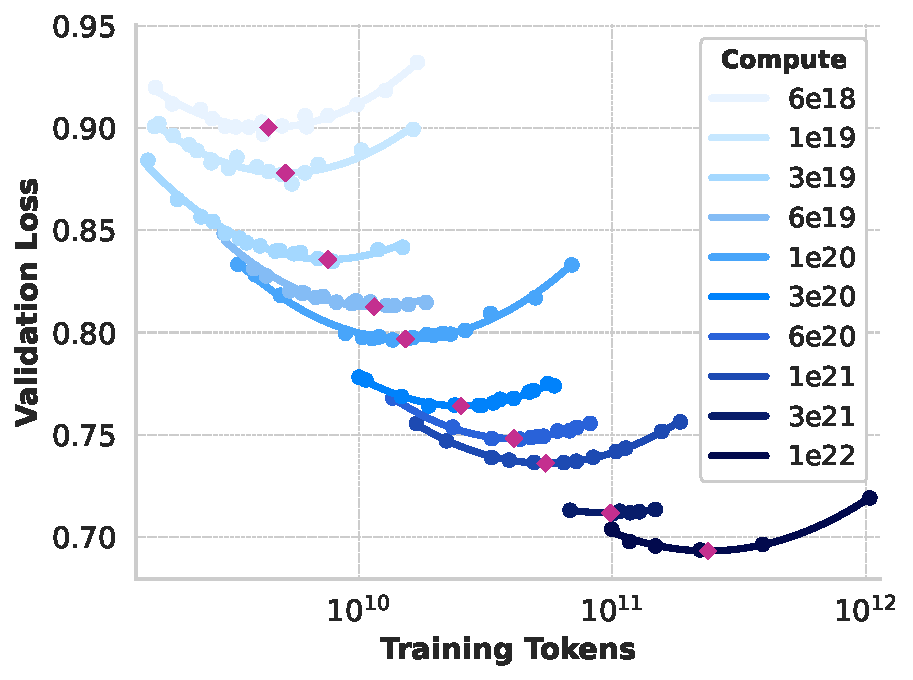
\includegraphics[width=0.9\textwidth]{assets/isoflops.pdf}
		\caption{\textbf{Scaling law IsoFLOPs curves} between $6 \times 10^{18}$ and $10^{22}$ FLOPs. The loss is the negative log-likelihood on a held-out validation set. We approximate measurements at each compute scale using a second degree polynomial.}
		\label{fig:scaling_law_isoflops}
	\end{minipage}\hfill%
	\begin{minipage}{0.45\textwidth}
		\centering
		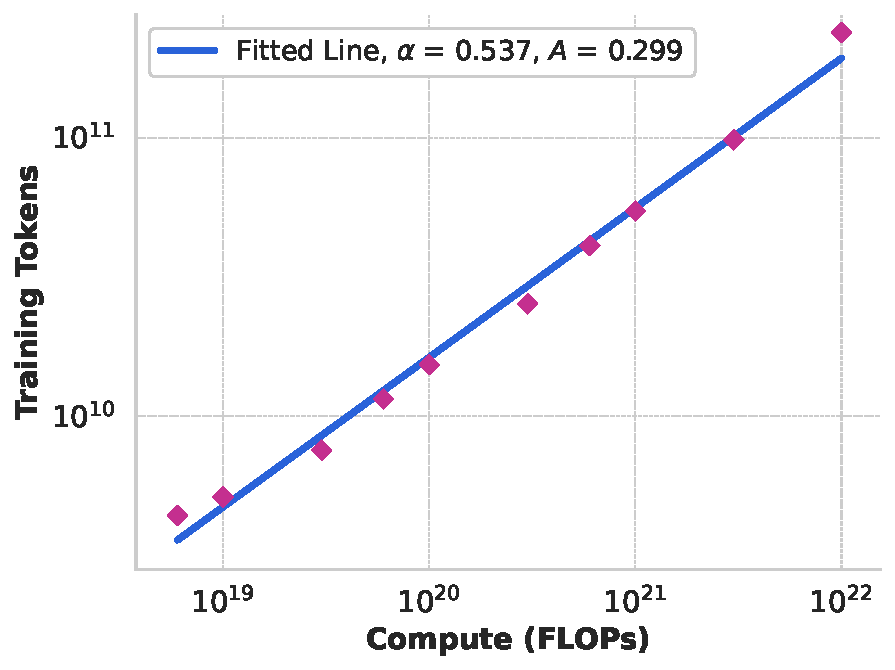
\includegraphics[width=0.9\textwidth]{assets/datacompute.pdf}
		\caption{\textbf{Number of training tokens in identified compute-optimal models as a function of pre-training compute budget.} We include the fitted scaling-law prediction as well. The compute-optimal models correspond to the parabola minimums in Figure~\ref{fig:scaling_law_isoflops}.}
		\label{fig:data_compute_scaling_law_fit}
	\end{minipage}
\end{figure}

These experiments give rise to the IsoFLOPs curves in Figure~\ref{fig:scaling_law_isoflops}.
The loss in these curves is measured on a separate validation set.
We fit the measured loss values using a second-degree polynomial and identify the minimums of each parabola.
We refer to minimum of a parabola as the \emph{compute-optimal} model at the corresponding pre-training compute budget.


We use the compute-optimal models we identified this way to predict the optimal number of training tokens for a specific compute budget.
To do so, we assume a power-law relation between compute budget, $C$, and the optimal number of training tokens, $N^\star(C)$:
\begin{align*}
    N^\star(C) = A C^\alpha.
\end{align*}
We fit $A$ and $\alpha$ using the data from Figure~\ref{fig:scaling_law_isoflops}.
We find that $(\alpha, A) = (0.53, 0.29)$; the corresponding fit is shown in Figure~\ref{fig:data_compute_scaling_law_fit}.
Extrapolation of the resulting scaling law to $3.8 \times 10^{25}$ FLOPs suggests training a
402B parameter model on 16.55T tokens.


An important observation is that IsoFLOPs curves become \emph{flatter} around the minimum as the compute budget increases.
This implies that performance of the flagship model is relatively robust to small changes in the trade-off between model size and training tokens.
Based on this observation, we ultimately decided to train a flagship model with 405B parameters.


\textbf{Predicting performance on downstream tasks.} We use the resulting compute-optimal models to forecast the performance of the flagship Llama 3 model on benchmark data sets. 
First, we linearly correlate the (normalized) negative log-likelihood of correct answer in the benchmark and the training FLOPs. In this analysis, we use only the scaling law models trained up to $10^{22}$ FLOPs on the data mix described above.
Next, we establish a sigmoidal relation between the log-likelihood and accuracy using both the scaling law models and Llama 2 models, which were trained using the Llama 2 data mix and tokenizer.
We show the results of this experiment on the ARC Challenge benchmark in Figure~\ref{fig:scaling_law_benchmarks}).
We find this two-step scaling law prediction, which extrapolates over four orders of magnitude, to be quite accurate: it only slightly underestimates the final performance of the flagship Llama 3 model.

\begin{figure}[tbp]
	\centering
	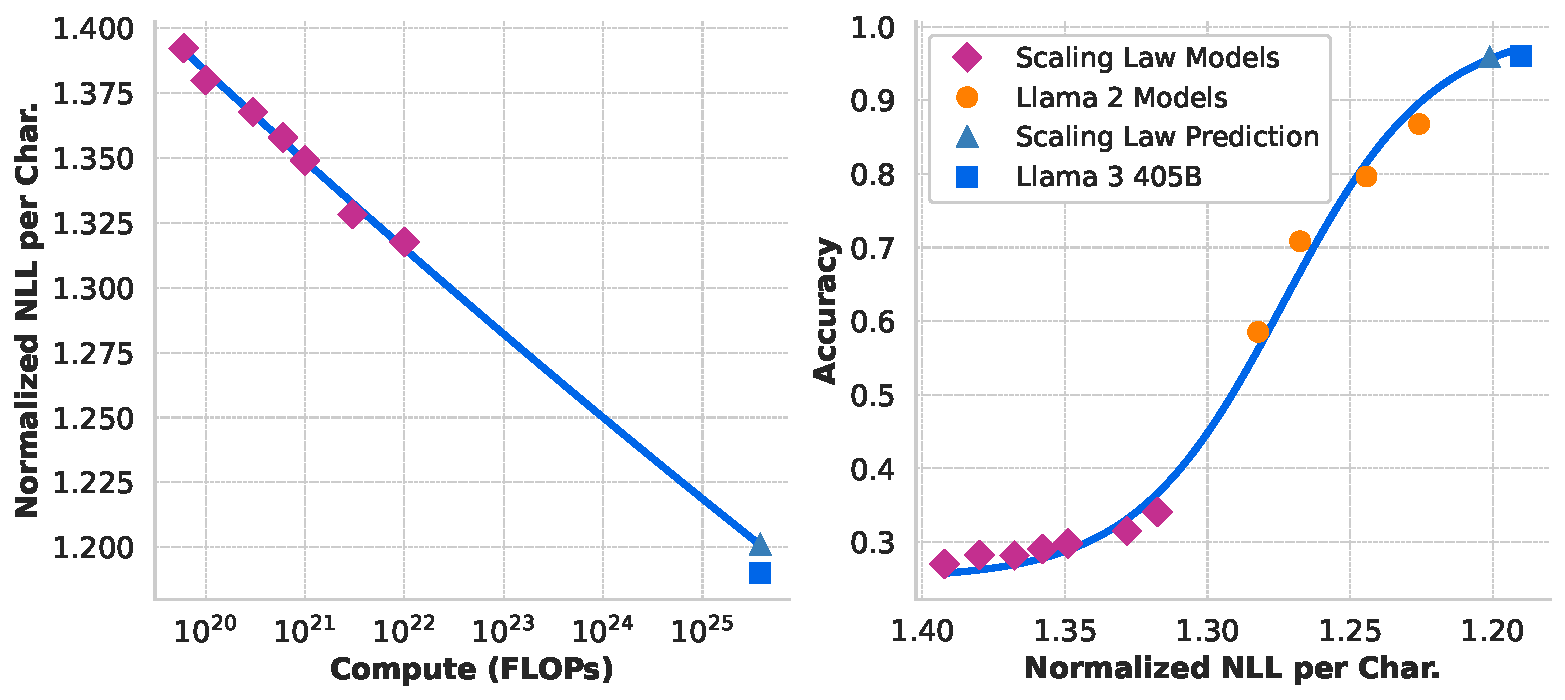
\includegraphics[width=0.7\textwidth]{assets/scaling_laws_benchmark.pdf}
	\caption{\textbf{Scaling law forecast for ARC Challenge.} \emph{Left:} Normalized negative log-likelihood of the correct answer on the ARC Challenge benchmark as a function of pre-training FLOPs.
	\emph{Right:} ARC Challenge benchmark accuracy as a function of the normalized negative log-likelihood of the correct answer. This analysis enables us to predict model performance on the ARC Challenge benchmark before pre-training commences. See text for details.}
	\label{fig:scaling_law_benchmarks}
\end{figure}
